%!TEX root = ..//preambulo.tex

\section{Material e Método}

 \subsection*{Local de Estudo}


  \hspace*{1.25 cm}  A região estudada está localizada na microrregião administrativa central do estado do Espírito Santo, próxima ao delta do rio Doce, em uma planície fluvial composta por depósitos quaternários, dividida em porções de natureza lagunar e fluvial, ambas caracterizadas por processos de acumulação. Os solos predominantes na área incluem Cambissolos Eutróficos e Organossolos, sem influência marinha.\\
  %
     \begin{wrapfigure}{r}{0.50\textwidth}
	\begin{center}
		\centering \small \caption{Zona hachurada, região da repactuação}
		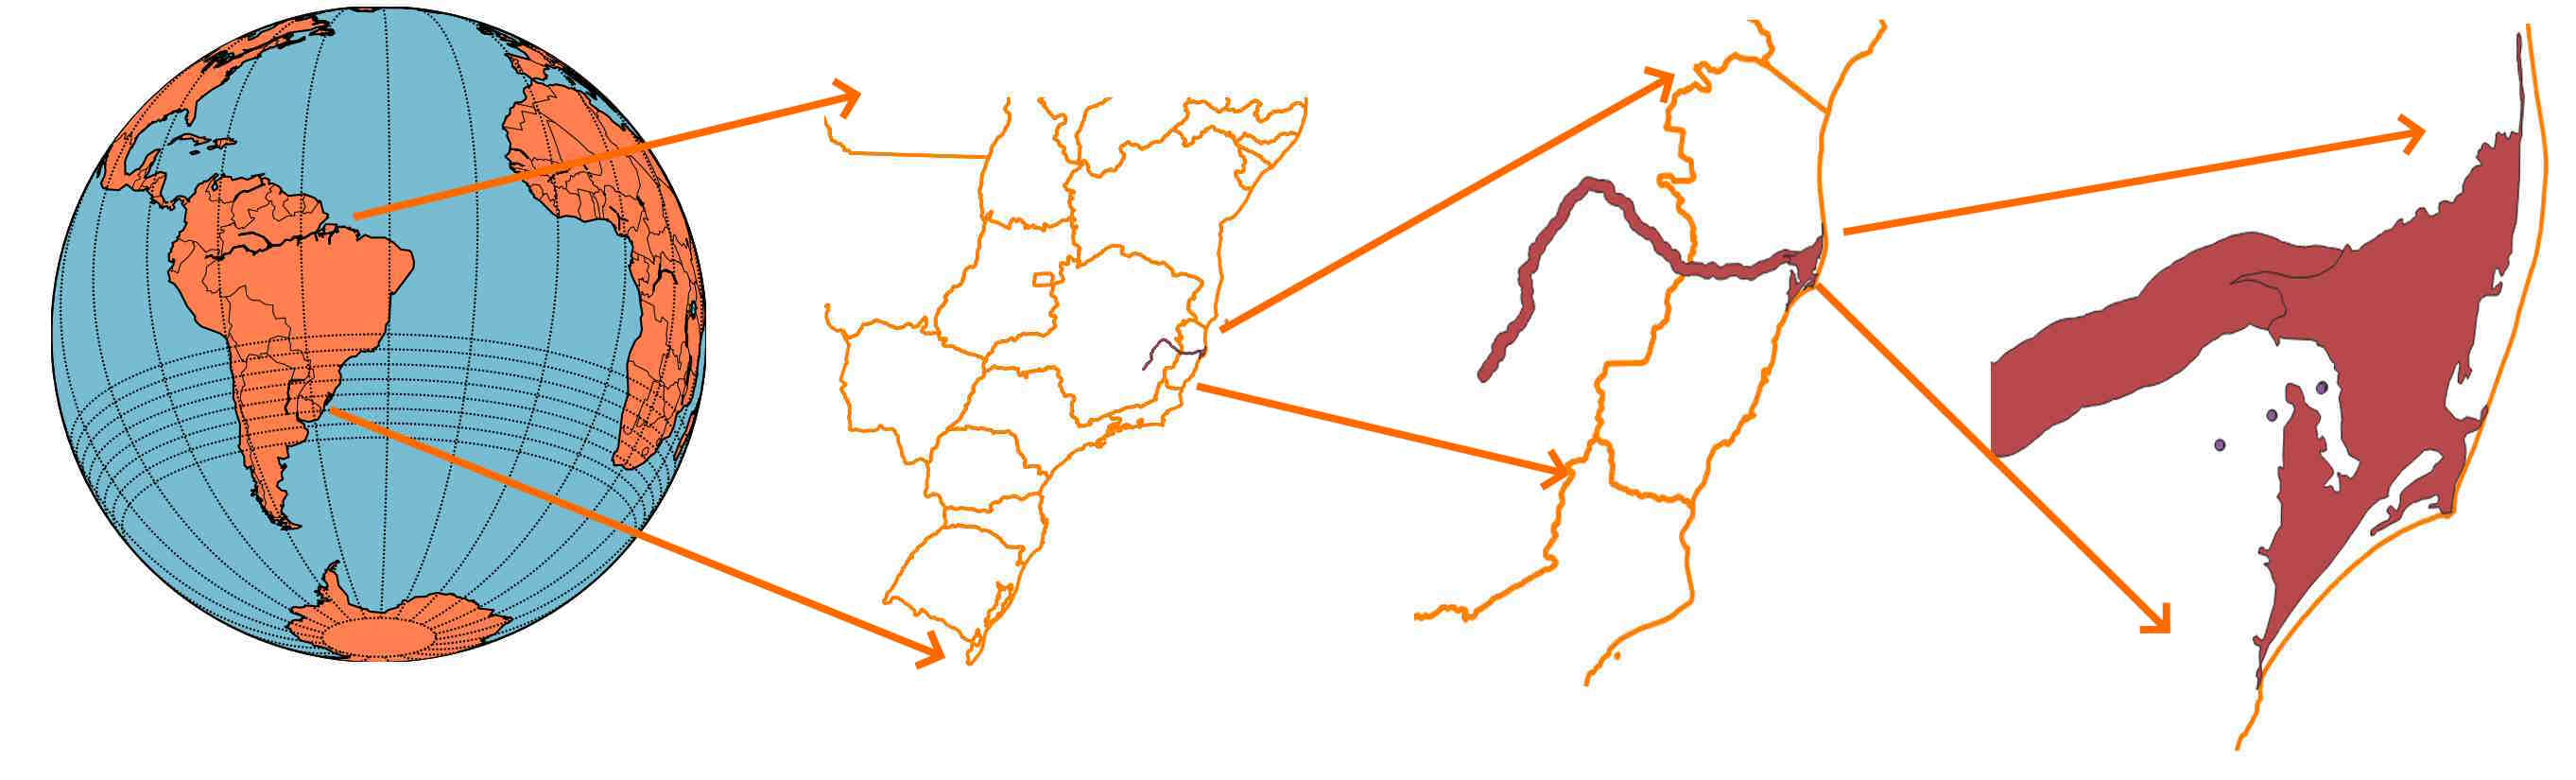
\includegraphics[width=0.96\linewidth]{FIGURAS/Localizacao}
		\label{fig:localizacado}\\{Fonte: Elaborado pelos Autores (2025)}
	\end{center}
\end{wrapfigure}
  \hspace*{1.25 cm}  O relevo da região é predominantemente plano, com declividade inferior a 2\% em toda a sua extensão. Quanto ao uso do solo, podem ser identificadas seis classes principais: (1) áreas de cultivo com culturas como mamão, coco-da-baía, cana-de-açúcar e abacaxi, entre outras; (2) áreas de reflorestamento, em proporção semelhante às áreas cultivadas; (3) pastagens; (4) brejos; (5) porções esparsas de solo exposto; e (6) pequenas áreas de corpos d’água, como açudes. \\
  %
%
  %
  \hspace*{1.25 cm} A escolha desta região como objeto de estudo justifica-se pela diversidade de usos do solo mencionada, que permite a análise da área sob a perspectiva da repactuação ambiental. Além disso, a região possibilita a observação de eventos climáticos extremos, como inundações (conforme ilustrado na Figura \ref{fig:indao}), e o estudo do encontro do fluxo de rejeitos com a foz do rio Doce e o oceano Atlântico, destacado nas figuras correspondentes. \ref{fig:indao2} e \ref{fig:indao3}\\  
% {{{   
			\begin{minipage}[t!]{0.33\textwidth}
				\begin{figure}[H]
					\centering \small \caption{Ano de 2013}
					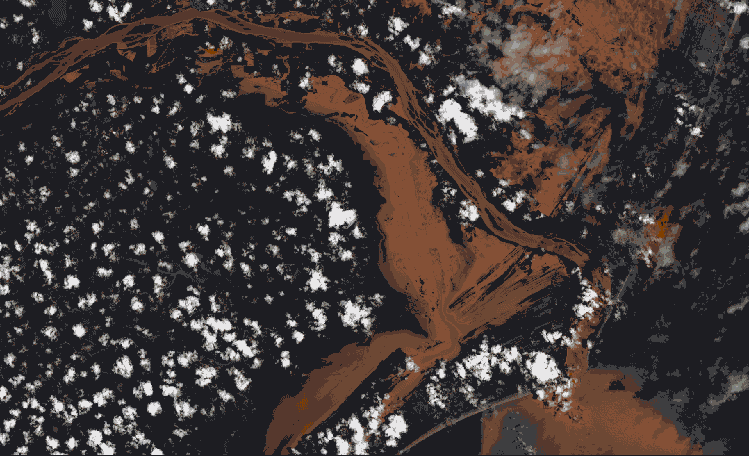
\includegraphics[width=0.97\linewidth]{FIGURAS/20131226-compr}
					\label{fig:indao} 
				\end{figure}			
			\end{minipage}\hfill
			\begin{minipage}[t!]{0.33\textwidth}
				\begin{figure}[H]
					\centering \small \caption{Ano de 2016}
					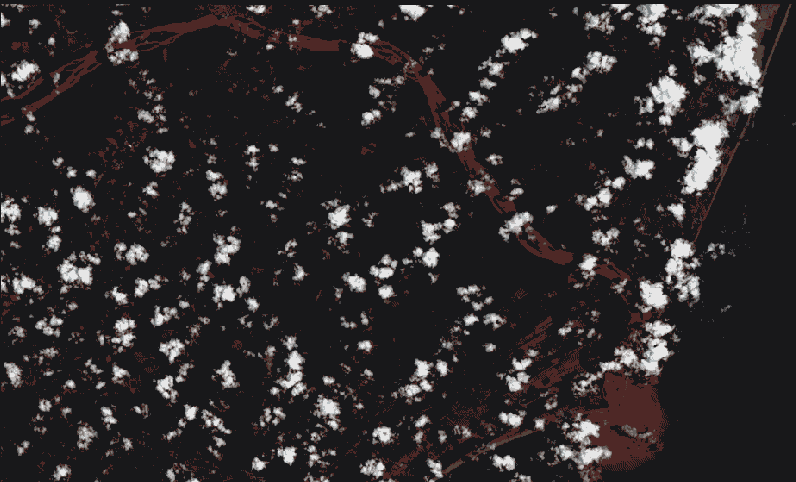
\includegraphics[width=0.97\linewidth]{FIGURAS/20160202compre}
					\label{fig:indao2} 
				\end{figure}					
			\end{minipage} 
			\begin{minipage}[t!]{0.33\textwidth}
				\begin{figure}[H]
					\centering \small \caption{Ano de 2016}
					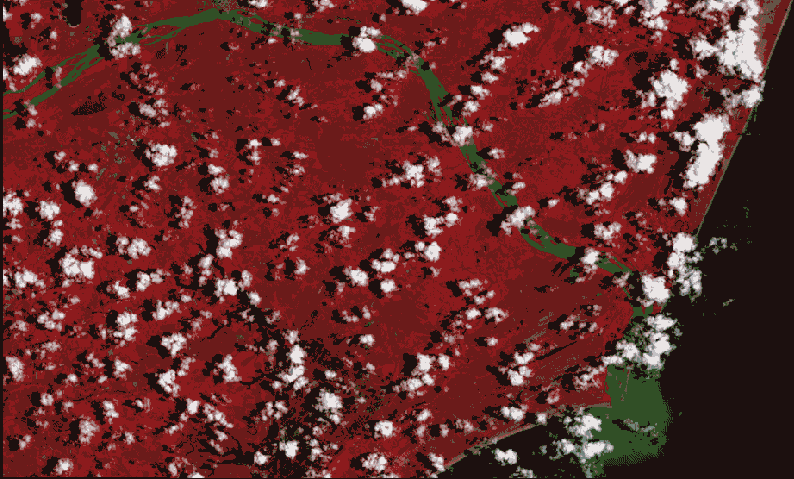
\includegraphics[width=0.97\linewidth]{FIGURAS/20160202rcompre}
					\label{fig:indao3} 
				\end{figure}					
			\end{minipage} 
			\begin{center}
				Fonte:   Elaborado pelos Autores (2025)
			\end{center}
			% }}}

  \hspace*{1.25 cm} Com base na análise da situação física e considerando que o objeto da repactuação abrange uma área de 5.723,26 km², o local de estudo aprofundado corresponde a uma extensão de 10.000 hectares. Assim, o instrumento mais adequado para a pesquisa é o uso de imagens aéreas ou orbitais, com preferência por estas últimas. O delineamento da pesquisa será amostral, de caráter qualitativo-descritivo, com a variável mensurada longitudinalmente em um painel temporal\\
  %
    \hspace*{1.25 cm} Para minimizar questionamentos técnicos ou sociais, a metodologia deve ser delineada de forma totalmente replicável, tanto em sua estrutura quanto em seu conteúdo. A base teórica será fundamentada, majoritariamente, em publicações internacionais, como livros e artigos científicos. As imagens utilizadas como base de dados serão disponibilizadas gratuitamente à comunidade científica. Além disso, os aspectos substantivos serão priorizados, com afirmações fundamentadas em resultados matemáticos. Por fim, a pesquisa adotará uma abordagem adjetiva, classificando a situação antes, durante e após o evento extrínseco.

 \subsection*{Sensoriamento Remoto}

  \hspace*{1.25 cm} A obtenção de dados obtidos por sensoriamento remoto, o principio básico de sensoriamento remoto, disposto por \cite[p.~24]{Reddy} é "ciência e a arte de se obter informação sobre um objeto, área ou  fenômeno o através de uma analise de dados adquiridos sem o contado com o objeto, fenômeno que se está sendo investigado".  Acrescenta-se ainda que em \cite[p.~7]{Jensensens} descreve que além das coordenadas x,y,z e profundidade , o sensoriamento remoto possibilita a analise da biomassa, a temperatura, e suas misturas contidas, e ainda outras. \\
  %
  \hspace*{1.25 cm} De mesma forma em \cite[p.1]{Lilesat} :
   \begin{quoting}[rightmargin=0cm,leftmargin=4cm]
 	\begin{singlespace}
 		{
 			\textit{A ciência e arte de obter informações a respeito de um objeto, área ou fenômeno pela análise de dados adquiridos por um sistema que não se encontra em contado com o objeto , área ou fenômeno sob investigação}
 		}
 	\end{singlespace}
 \end{quoting}
 \hspace*{1.25 cm} A captação dessas informações, ocorre por meio de dados, reflectividade do objeto observado - superfície terrestre -, ocasionado pela emissão de energia eletromagnética emitida pelo sol, sendo parte absorvida pela  superfície terrestre e parte reflectida a atmosfera. e em ambos efeitos são  captados  por sensores orbitais.\\
 %
  \hspace*{1.25 cm} Diferentes sensores, com atributos e processos construtivos diferentes e  inerentes, segundo \cite[p.~20]{Centeno} armazenarão o espectro eletromagnéticos, comprimento de ondas de variável contínua, em canais e/ou bandas especificas. Esses canais, comprimento de ondas em faixa distintas divididas e  classificadas, a partir deste momento em variável discreta,  são denominadas \textbf{\textit{resolução espectral}}, ainda em \cite[p.~54]{Centeno} a maior ou menor capacidade de registrar diferenças espectrais entre os alvos e a medida desejada. Considerando as perdas atmosféricas, variações temporais, e as propriedades inerentes dos corpos imageados; composições químicas. \\
%
  %
  \hspace*{1.25 cm} O processo  de manipulação e classificação da variável discreta e seu espaço multidimensional e sua coordenada  \textbf{DN(x,y) }, como em \cite[p.~183]{Schowengerdt}, possui nome próprio denominado em linguá inglesa  "\textbf{\textit{Spectral Tranforms}}". E dentro destas operações matemáticas para se obter melhorias da informação destas imagens, agora em \cite[p.~485]{Lilesat}, sejam estas operações: manipulação de contrastes, correções geométricas, correções radiométricas , classificação entre outras. Existe um processo a ser desenvolvido neste estudo, denominada diferenças normalizadas e índices.\\
%
%
 \hspace*{1.25 cm} Voltando a \cite{Centeno} e este citando \cite[p.339]{Chuvieco}, é a combinação entre bandas, obtendo uma nova imagem, com características distinta, de forma a realçar a informação dos alvos e suas variações químicas e bióticas. \\
%
\hspace*{1.25 cm} Esta imagem, georreferenciada, mesmo sem o processo de classificação automática ou manual, pode ser entendida em estar em  perspectiva tri-dimensional (3d) por banda com características (x,y, valor discreto), mas pode incorporar  a quarta dimensão (4d) o tempo.
\begin{figure}[H]
	\centering  \small \caption{Quatro dimensões  em cubo de dados : x,y,banda, e tempo}
	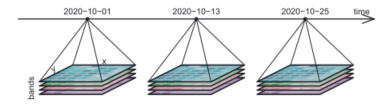
\includegraphics[width=0.97\linewidth]{FIGURAS//quatroDimensao}
	%\caption{\href{file:./DIAGRAMAS/flow-diagrama-Alterado2.tex}{TEX File} }
	\label{fig:quatroDimensao}{ Fonte:  Em \cite[p.60]{Pebesma} }
\end{figure}
  \hspace*{1.25 cm} A partir do conceito, que compreendemos como cubo de dados, deve-se ter em mente que a variação da atributo do objeto a ser mensurado, este deve ser coletado. Então  surge a necessidade de amostragem, melhor dizendo, um plano de amostragem, livre de vieses , este detectando a variedade temporal, em sua estrutura de posicionamento, incluindo a principal variedade medida, que em nosso caso é a reflectância e suas composições e combinações .
%
%
 \subsection*{Amostragem}
 %
            \begin{wrapfigure}{l}{0.65\textwidth}
 	\begin{center}
 		\centering  \small \caption{Amostragem em classes}
 		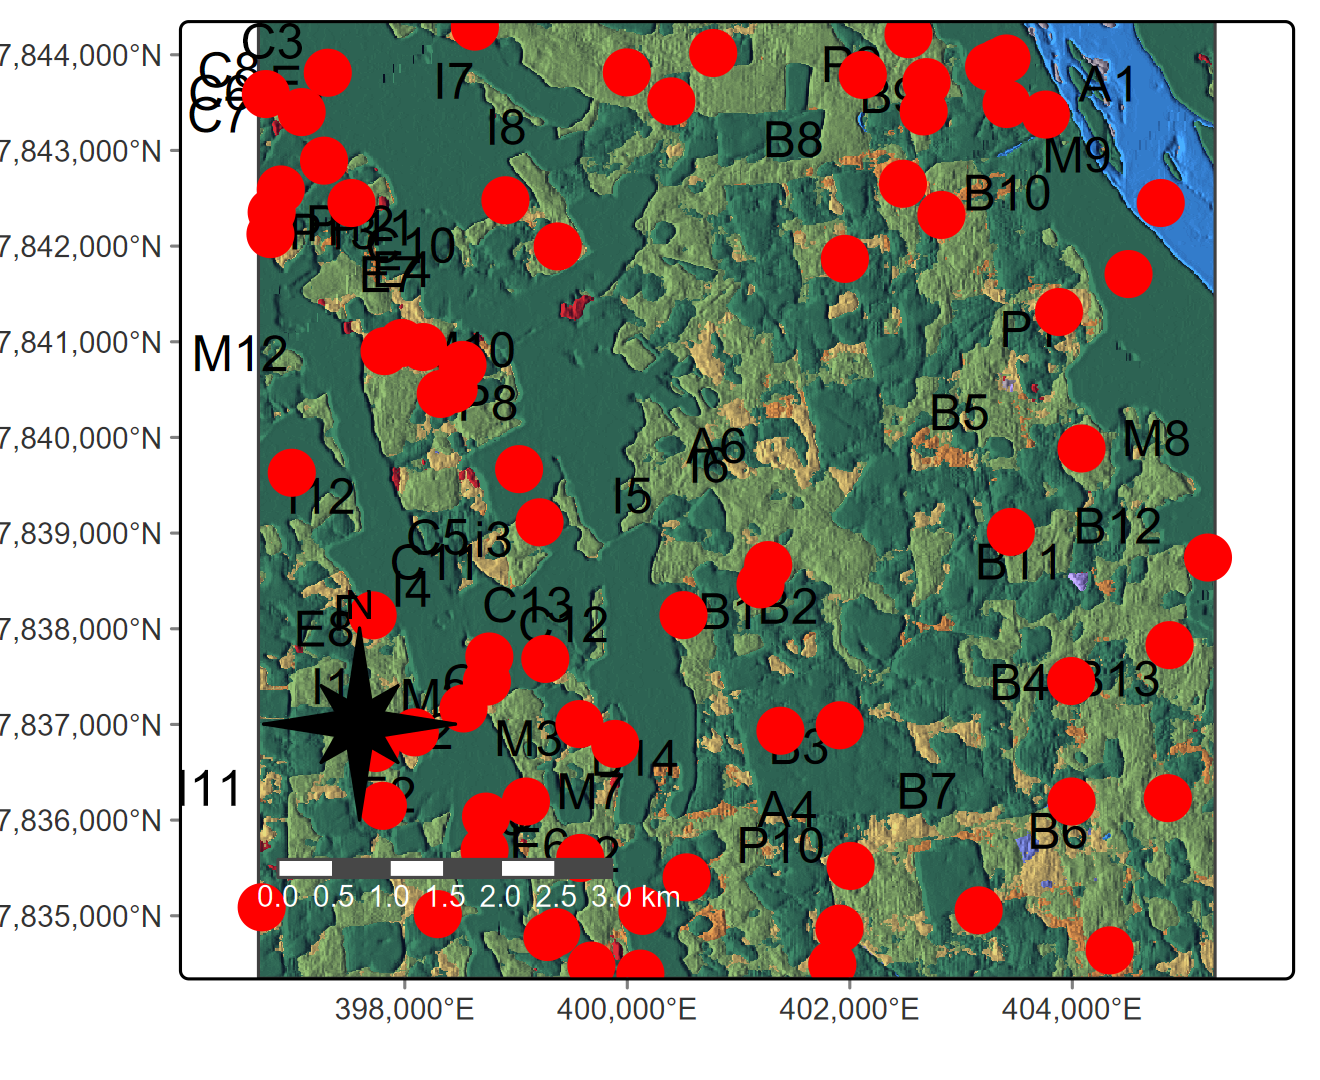
\includegraphics[width=0.97\linewidth]{FIGURAS/usoSOLOamostras}
 		\label{fig:usoSOLOamostras}\\{ Fonte:   Elaborado pelos Autores (2025)}
 	\end{center}
 \end{wrapfigure} 
  \hspace*{1.25 cm} O conceito de amostragem, e mais especificamente uma amostra, para  \cite[p.~281]{Krishnaswamy} deve ser utilizado quando \textbf{\underline{não é possível}} ou prático utilizar observação do fenômeno estudado em toda a população, este empecilho pode ser ocasionado por diferentes formas, sejam ele associados a localização geográfica, população numerosa, ou mesmo custo de aquisição elevado.\\
 %
 %
  \hspace*{1.25 cm}  Acrescenta-se a estes fenômenos, temos o tempo, pois se a alteração já ocorreu existe a dificuldade de rever eventos que foram alterados,e por isso devemos ter métodos de obtenção desta informação na época estuda, e por isso utilizamos ás técnicas de sensoriamento remoto, e processamento de imagem  para obtermos a informação.\\
  %
    %
  \hspace*{1.25 cm} E ao estabelecimento do plano de amostragem, devemos ter em mente o conceitos de esta atividade o  \cite[p.2]{Bolfarine1},  o pesquisador planeja, executa, corrige e analisa o procedimento a ser proposto e usado. Tendo como base a técnica de mensuração, e a questão respondida.\\
% 
 %
  \hspace*{1.25 cm} A escolha do método de amostragem livre de viés, e que o erro de estimativa seja minimizado, está diretamente ligado a estrutura de amostragem.  Em nosso estudo optamos primeiramente pela estratificada aleatória por classe de uso do solo, de acordo com \cite[p.191]{Ariza}, e  posterior  de  sistemática, estabelecimento de um \textbf{grid}, por grades regulares.\\
  %
   %
  \hspace*{1.25 cm}  O objetivo da primeira técnica, segundo  \cite[p.22]{Lohr} quando o tipo de amostragem por estratificação pode ser utilizada em regiões especificas que desejamos obter informação, em nosso caso a variação de reflectância temporal em classes de uso do solo especifica. Já na segunda  possibilitando que todos os fenômenos mensurados, tenham a mesma possibilidade de ser coletado.\\
  %


  %
 \hspace*{1.25 cm} A metodologia de planejamento e direcionamento baseada na relação entre amostras e classes de uso do solo é um procedimento comum entre profissionais da área de cartografia. Diversos estudos descrevem essas atividades; no entanto, segundo os autores, os trabalhos mais relevantes destacam os conhecimentos apresentados por Congalton \cite[p.79]{Congalton}, que vinculam cada classe de uso do solo à quantidade de amostras correspondente. Além disso, Ariza \cite[p.135]{Ariza} complementa ao determinar o tamanho amostral e o erro com base na estimativa, enquanto \cite[p.192-196]{Ariza} ilustra os quantitativos, em metros quadrados, de cada classe de uso do solo e o número necessário de fragmentos por classe. Esses fundamentos permitem a aplicação de fórmulas estatísticas, como a equação \( n= \dfrac{zC ^{2} * sd^{2}* N}{ E^{2}(N-1) + Zc^{2}*sd^{2}} \) para determinar o número de amostras por classe, considerando o erro, o nível de confiança estipulado e a representação gráfica demonstrada na Figura \ref{fig:usoSOLOamostras}  .\\
 %
   %  \hspace*{1.25 cm}  Segundocorroborando a escolha do plano de amostragem estratificada, em outros termos: segmentação de grupos em estratos(ou subpopulações),  é o conhecimento prévio da área de estudo, possibilitando que as amostras sejam suficiente e se destaque eventos mais importantes.\\
    

  \subsection*{Geoestatística} 

 \hspace*{1.25 cm} Segundo \cite[p.1]{delgado}  a modelagem geoestátistica, tem um papel chave na análise da evolução de eventos distribuídos sobre a superfície da terra e ciências da engenharia ligadas a recursos naturais. \\
 %
   \hspace*{1.25 cm} A  utilização de malha regularas, também conhecido como "\textbf{grid}" , como exposto em \cite[p.83]{Andriotti}, tem a função de através de pontos amostrados, estabelecer um mapa de forma continua, passível de estimar valores dentro deste estrutura e até estabelecer extrapolações. Isso é possível através de técnicas de interpolação, voltando a \cite[p.304]{Ariza},  caracterizando o papel da interpolação, para este autor, "\textit{a interpolação e uma transformação que permite estivar valores desconhecidos a partir de valores conhecidos em posições certas}". \\
  %
    \hspace*{1.25 cm} Isso ocorre por que, conforme \cite[p.21]{Yamamoto}, o fenômeno espacial compreende um conjunto de valores possíveis da variável de interesse, e a sua distribuição e variabilidade está dentro de respectivos domínios sejam eles 2D ou 3D.  Voltando a  \cite[p.95]{Andriotti}, pode ser caracterizada como variável regionalizada.\\
  %
  \hspace*{1.25 cm}  Em  \cite[p.37]{Webster} os fenômenos físicos naturais, possuem variação determinística e sistemática, e estão relacionados a campo da matemática e geometria. E através destas das técnicas, podemos estabelecer predicações e interpolações entre elas a polígonos de Thielsse, inverso da distancias, superfícies de tendencias, splines e por fim a krigagem.   
  %
  \subsection*{Dados Espaço - Temporal} 
  
  %
  \hspace*{1.25 cm} O paradigma espaço tempo, para \cite[p.2]{mateu}, este processo pode ser assumido como um modelo estatístico, e ser representado pela equação:
  \begin{equation}
  	 Z(x,s,t) =  \eta ( x,(s,t), s.t.\beta) + \in (x,s,t)  \; s \in D, t \, \in T.  
  \end{equation}
  %
  \hspace*{1.25 cm}   Onde $s$ corresponde a uma localização espacial, $t$ um momento temporal, $x$ potencialidades  dependentes de regressões , e $ \eta $ uma parametrização do modelo.\\
  %
   \hspace*{1.25 cm} Para outro autor,  \cite[p.151]{Bivand} o interesse e local estudado, pode ser separado em: ponto ou área, tempo ou intervalo, e por fim a ocorrência medida. Já que possuem diferentes  propriedade e qualidade também distintas  \\
   %
  \hspace*{1.25 cm} A etapa inicial consiste na obtenção de dados (imagens), que podem ser adquiridos por meio de plataformas como o Google Earth Engine (GEE), agilizando o processo de produção de informações. Esses dados podem ser integrados à implementação de scripts que automatizam a busca por cenas em datas específicas, permitindo também o cruzamento com outras informações para análises mais precisas, como a avaliação da cobertura e uso do solo atual (Figura \ref{fig:area-de-estudo}). Além disso, é possível selecionar aspectos como o percentual de cobertura de nuvens e o intervalo espaço-temporal das informações obtidas.
  %
  %
  \lstset{
  	language=Java, % Define a linguagem como JavaScript
  	caption=Código de obtenção de imagens multiespectrais Landsat8 plataforma Google Earth Engine Code\, em linguagem JavaScript.,} % Legenda do código
  
  \begin{lstlisting}
  	var dataset = ee.ImageCollection('LANDSAT/LC08/C02/T1_L2')
  	.filterDate('2013-05-01', '2025-05-01');
  	// Applies scaling factors.
  	function applyScaleFactors(image) {
  		var opticalBands = image.select('SR_B.').multiply(0.0000275).add(-0.2);
  		var thermalBands = image.select('ST_B.*').multiply(0.00341802).add(149.0);
  		return image.addBands(opticalBands, null, true)
  		.addBands(thermalBands, null, true);   	}
  	dataset = dataset.map(applyScaleFactors);
  	var visualization = {
  		bands: ['SR_B4', 'SR_B3', 'SR_B2'],
  		min: 0.0,
  		max: 0.3,  	};
  	Map.setCenter(-39.93696, -19.5597, 8);
  	Map.addLayer(dataset, visualization, 'True Color (432)');
  \end{lstlisting}
 %=========================================================== 
  \subsection*{Operações}  
 \hspace*{1.25 cm} A operação com dados raster, dados binários, para \cite[106]{Dormam} "\textit{grids de valores numéricos}", e estes estão agrupados bandas espectrais, e para \cite[p.178 e p.181]{Liu}  podem sofrer operações e conversões unárias, e sujeitas a operações comuns matemáticas com: adição, subtração, multiplicação, divisão, módulos. Inclui-se também operações relacionais e boleanas, logicas e combinatórias.  \\
 %
 \hspace*{1.25 cm}  Neste contexto, inicia-se nossas atividades. A compreensão de índices espectrais, devemos entender, que são operações matemáticas entre bandas, sendo amplamente difundidos em diferentes meios das literatura técnica. Ao nosso estudo de alteração do meio físico, e conhecendo que os principais elementos encontrados no local são: solo, a água e a vegetação, entende-se  que  os índices  são capazes meios capazes de ser sensibilizados pelas variações destes elementos. E ao utilizamos as operações algébricas  1, 2, e 4 , de combinação de bandas que estão dispostas em \cite[p.165]{Thekapbail} e equação 3 \cite[p.7]{Thekapbail}. 
 %
 \begin{equation}
 	 NDVI = \dfrac{nir - red}{ (nir + red) }
 \end{equation}
 \begin{equation}
	NDWI = \dfrac{green - nir}{ (green + nir) }
\end{equation}
 \begin{equation}
	EVI = \dfrac{G*(nir - red)}{ nir + 2,4. red +1) }
\end{equation}
 \begin{equation}
	SAVI = \dfrac{(nir - red)*(1 +l)}{ (nir + red +L) }
\end{equation}
%
\hspace*{1.25 cm} Onde, "red" corresponde a banda vermelha, "green" a banda verde, "NIR" o infra vermelho proximo, e o "L" correção de reflectâncias do solo.\\
%
 \hspace*{1.25 cm} Para manipulação destes dados utilizando a linguagem R na versão 4.5, e ambiente de desenvolvimento junto ao notebook Jupyter, somente devido ao ambiente gráfico junto ao navegador de internet, em termos corretos são chamados em lingua inglesa de "browser", mesmo sendo possível realizar todas as operações junto ao RStudio 2015.05. Necessitamos esclarecer que  todos as bibliotecas no R são chamadas de "package, e ao carregarmos o pacote, " \textbf{\textcolor{blue}{raster}}" e "\textbf{\textcolor{blue}{terra}}", ao software pelo comando.
   \lstset{
 	language=R, % Define a linguagem como JavaScript
 	caption=Código para carregar imagens   em linguagem R,} % Legenda do código
\begin{lstlisting}[language=R]
library(raster)
library(terra)
raster_template <- terra::rast("D:\\IMAGENS2\\lc_20160202.tif")	   
\end{lstlisting} 
 \hspace*{1.25 cm} O package "RSToolsBOX", atualmente na versão, 1.0.2.1, traz uma serie de ferramentas para trabalharmos com dados de sensoriamento remoto, tanto que este vem incorporado com as funções e/ou equações matemáticas nas 1 a 4. E dentro destas funções temos a função  "\textbf{\textcolor{blue}{spectralIndices}}", usada no script a seguir :
%
   \lstset{
	language=R, % Define a linguagem como JavaScript
	caption=Código para obter índices  em linguagem R,} % Legenda do código
\begin{lstlisting}[language=R]
VI_20131023 <- spectralIndices(raster_template, blue = "Layer_1", gree = "Layer_2" ,red = "Layer_3", nir = "Layer_4",swir2 =  "Layer_5", indices = c("NDVI", "NDWI","EVI2", "MSAVI") 
VI_palette <- brewer.pal(n = 10, name = "Spectral")
spplot(VI_20131023, col.regions = VI_palette, cuts = 6, col = "transparente")
\end{lstlisting} 
%
 \hspace*{1.25 cm} Este procedimento, visto que as duas imagens estão georreferenciadas ao mesmo sistema  de coordenadas, é observarmos por meios matemáticos a variação da reflectividade do mesmo ponto, por índices físicos medidos pelo sensor remoto, diminuindo a subjetividade do observador, e ao mesmo tempo qualificar e variância temporal da superfície.\\
 %
 %   
 \hspace*{1.25 cm} Tendo a imagens \ref{fig:ima2013} a  \ref{fig:inda2023}, estas em nível de cinza, e iniciarmos operações algébricas de obter diferenças entre duas imagens temporais em Figuras \ref{fig:rplot-ndwi2016} a \ref{fig:difer202332026}. \\
 %
 %
\hspace*{1.25 cm}  O próximo passo, ao inserir o "grid", malha regular espaçada a 1.600(mil e seiscentos ) metros, para iniciar as operações de interpolação. Duas respostas desejamos obter nesta etapa,  uma superfície continua, e uma superfície que seja possível demonstrar direções do fenômeno estudado. \\
% 
\hspace*{1.25 cm} De forma complementar, possibilite maneira de validação cruzada verificar as reflectâncias de classes discriminadas do uso do solo, estão aderente ao modelo. E por isso as técnicas de interpolação com métodos geoestatísticos se completam.\\
 % 
 \hspace*{1.25 cm} Inseridos os vértices do grid, pela biblioteca(package) \textbf{\textcolor{blue}{sp}}, quase todas as ferramentas para interpolação tem como passo fundamental o carregamento e perfeito funcionamento da biblioteca \textbf{\textcolor{blue}{stars}} e mais especificamente o \textbf{\textcolor{blue}{gstat}}, Posto que a interpolação ocorre entre a coordenadas geográfica e o valor mensurado. Além do mais, que este possibilita realizarmos a interpolação pelo inverso das distância, superfícies de tendência e krigagem.  O procedimento no R é: 
 \lstset{
	language=R, % Define a linguagem como JavaScript
	caption= Interpolação em linguagem R,} % Legenda do código
\begin{lstlisting}[language=R]
	library(stars)
	library(gstat)
	interpolado <- gstat::gstat(formula= variavelmensurada~1, locations = arquivodogrid, set = parametrosdomodelo )	 
	MDT <- raster::raster::raster("folder/mdtarquivo.tif", values = FALSE)  
\end{lstlisting}  
 % 
\hspace*{1.25 cm}  A ultima linha acima, é a incorporação do modelo digital de terreno, sendo este aconselhável ao realizarmos a krigagem e superfícies de tendencia.\\
 % 
\hspace*{1.25 cm}  O resultado deste modelo, uma superfície continua, já nos possibilita termo o valor observado, o predito, seus resíduos, zscore, incluído suas coordenadas. Mais a possibilidade de monitorarmos a raiz do erro médio quadrado, e a estimativa da porcentagem da variação explicada $ R^{2}$.\\
%%
\hspace*{1.25 cm}  E neste momento, o processo torna-se interativo, testando os vários métodos de interpolação(simples interpolação, inverso das distância, inverso da distância com pesos ponderados, superfície de tendência e a krigagem). Enfatizando, por  termos os valores medido e estimado todos as medidas de variabilidade (media, mediana,moda, medidas de dispersão, distribuição de frequência ...)  \\
%
\hspace*{1.25 cm}  Profissionais que desenvolvem modelos matemáticos, muitas vezes apresenta a dificuldades em estabelecer as funções de transformação para normalizar seus dados. A inclusão  do package/biblioteca \textbf{\textcolor{blue}{bestnormalize}}, auxiliou demasiadamente em nosso modelo, realizando suas estimativas automaticamente. A sua implementação a liguagem R procedeu-se:
 \lstset{
	language=R, % Define a linguagem como R
	caption= normalizacao do modelo em linguagem R,} % Legenda do código
\begin{lstlisting}[language=R]
 library(bestNormalize)
modelo_normal <- bestNormalize(arquivodogrid$variavelmensurada )
\end{lstlisting}  
\hspace*{1.25 cm}  Segundo \cite[P.35]{Yamamoto} o termo variograma, ou semivariograma, ocorre um confusão terminológica de acordo com a literatura utilizada, para estes autores preferimos o exposto por \cite[p.228]{Ferreira}.  \begin{quoting}[rightmargin=0cm,leftmargin=2cm]
	\begin{singlespace}
		{
	\textit{Semivariogramas são modelos gráficos utilizados para se detectar o grau de dependência espacial entre dados geográficos em diferentes intervalos de distâncias crescentes, predefinidos e contados a partir de uma posição espacial inicial qualquer. Este modelo se constitui na curva da função de variância y(h) dos dados, onde h é um intervalo de distância até uma origem arbitrária(.. )}
		}
	\end{singlespace}
\end{quoting}
%
\hspace*{1.25 cm} A  parcela da modularização dos nossos procedimentos e analise do variograma para nossos dados foram obtidos pelo código a seguir.  
 \lstset{
	language=R, % Define a linguagem como R
	caption= Producao do variogramas em linguagem R,} % Legenda do código
\begin{lstlisting}[language=R]
	library(gstat)
   variograma <- gstat::variogram(variavelmensurada~1, arquivodogrid)
\end{lstlisting}  
\hspace*{1.25 cm}  E por fim a krigagem agora utilizando o package, sendo os valores da listagem em  \textbf{\textcolor{blue!55!black}{automap}} que também faz de forma automatizada. start\_vals somente para apresentar no figura desejada.
  \lstset{
 	language=R, % Define a linguagem como R
 	caption= Produção da krigagem em linguagem R,} % Legenda do código
 \begin{lstlisting}[language=R]
   library(automap)
 variogram_auto <- autofitVariogram(variavelmensurada~1, arquivodogrid, start_vals=c(variogramar$nugget, variogramar$cov.pars[2], variograma$cov.pars[1]))
 \end{lstlisting}  
\hspace*{1.25 cm} Realizado a análise exploratória dos dados, estabelecido o modelo matemático que melhor se ajusta aos  fenômenos, podemos iniciar a inferência sobre nossos resultados. 
%   
   \begin{comment}
   \begin{wrapfigure}{r}{0.60\textwidth}
  	\begin{center}
  		\centering  \small \caption{Uso do solo em 2024}
  		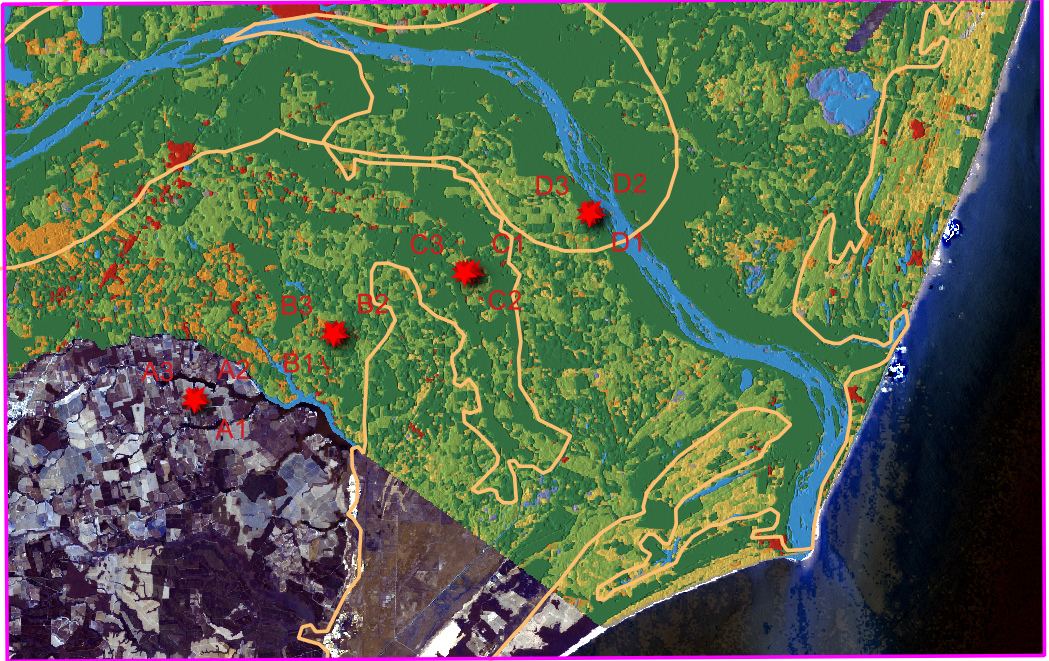
\includegraphics[width=0.97\linewidth]{FIGURAS/Area-de-estudo}
  		\label{fig:area-de-estudo} \\{ Fonte:   Elaborado pelos Autores (2025)}
  	\end{center}
  \end{wrapfigure}
    \end{comment}
     \begin{comment}
\begin{figure}[H]
		\centering  \small \caption{Fluxograma de procedimentos}
		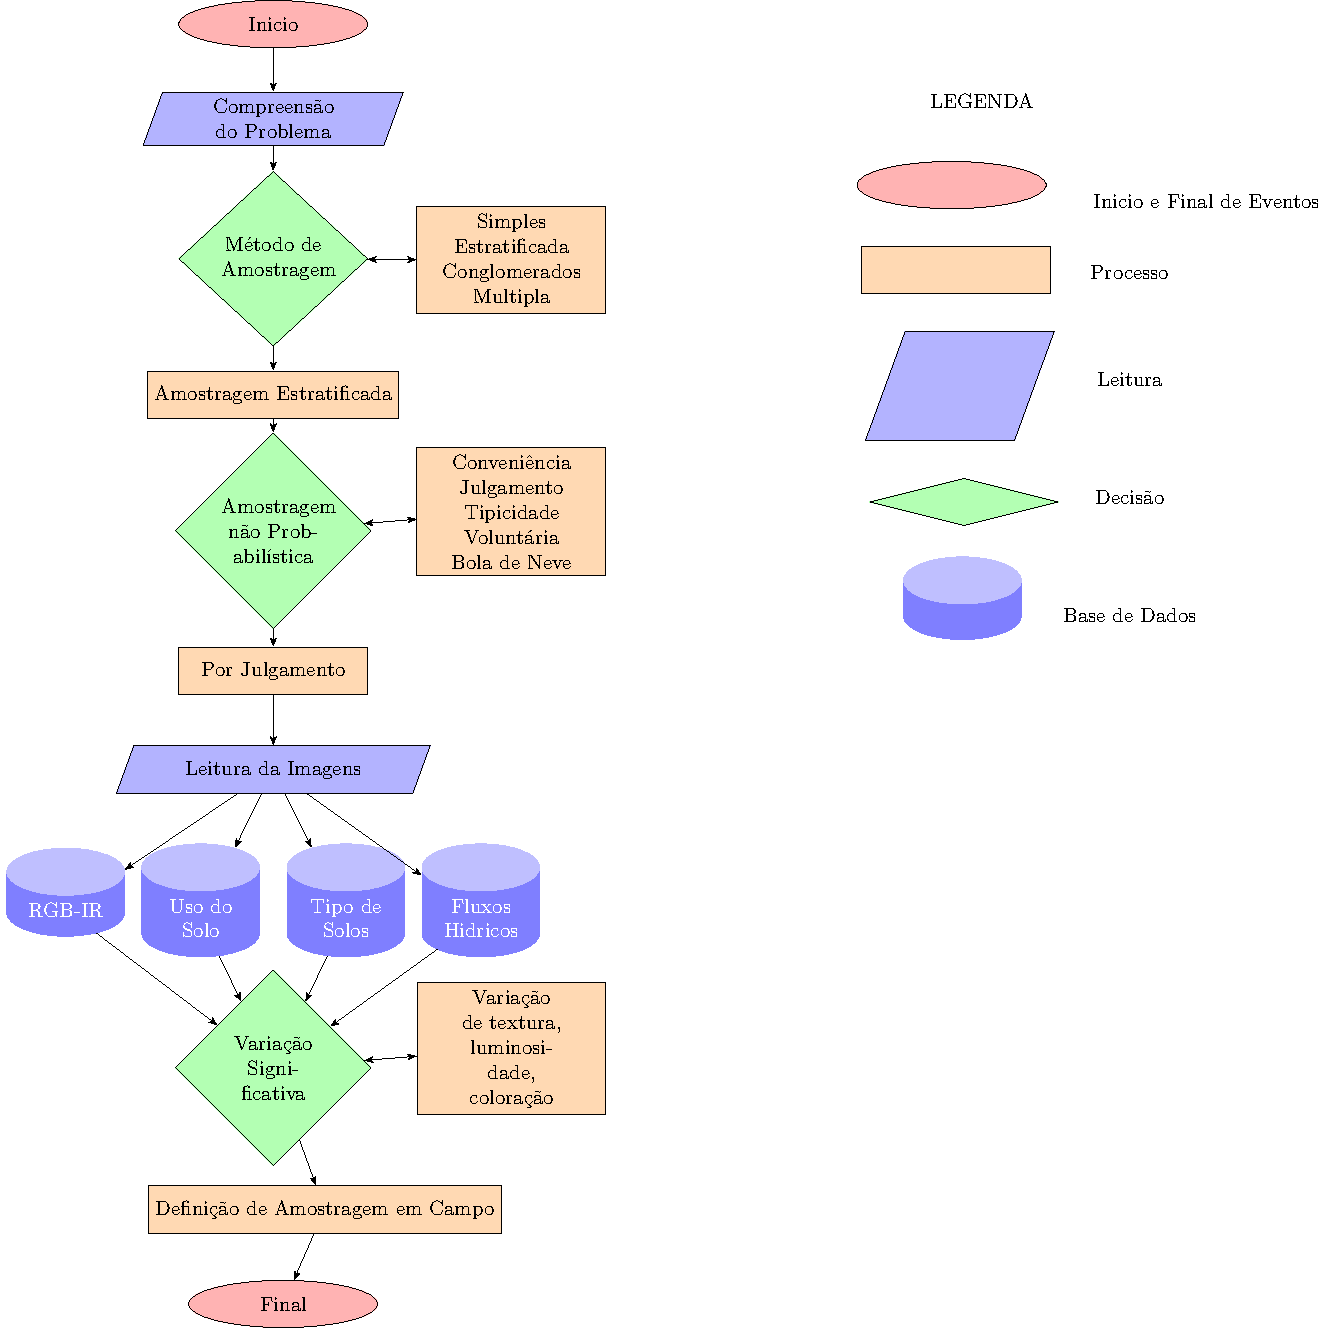
\includegraphics[width=0.47\linewidth]{DIAGRAMAS/flow-diagrama-Alterado2}
		%\caption{\href{file:./DIAGRAMAS/flow-diagrama-Alterado2.tex}{TEX File} }
		\label{fig:flow-diagrama-Alterado2}\\
		{ Fonte:   Elaborado pelos Autores (2025)}
\end{figure}  
        \end{comment}